\documentclass[a4paper, openany, 12pt]{article}

%% подключаем стандарт библиографии
\bibliographystyle{gost71u}

%% для "Abstract" в классе book
% \newenvironment{abstract}{}{}
% \usepackage{abstract}

%% подключаем преамбулу: в ней содержится подключение всех необходимых пакетов
%% Работа с русским языком
\usepackage{cmap}			 % поиск в PDF
\usepackage{mathtext} 		 % русские буквы в формулах
\usepackage[T2A]{fontenc}	 % кодировка
\usepackage[utf8]{inputenc}	 % кодировка исходного текста
\usepackage[russian]{babel}	 % локализация и переносы

%% Пакеты для работы с математикой
\usepackage{amsmath,amsfonts,amssymb,amsthm,mathtools}
\usepackage{icomma}

%% Нумерация формул (опционально)
%\mathtoolsset{showonlyrefs=true} % показывать номера только у тех формул, на которые есть \eqref{} в тексте.
%\usepackage{leqno}               % нумерация формул слева

%% Шрифты
\usepackage{euscript}	 % шрифт "Евклид"
\usepackage{mathrsfs}    % красивый мат. шрифт

%% Некоторые полезные макросы для дебага (в случае недоверия авторам шаблона)
\makeatletter
\newcommand\thefontsize{The current font size is: \f@size pt} % пример: \section{\thefontsize}
\makeatother

%% Настройка размеров шрифтов
\makeatletter
\setlength{\headheight}{28pt}
%% TODO: мне не удалось разобраться, как грамотно подбирать второе число в 
%% \@setfontsize\*, но ряд эксппериментов показывает, что "10" выравнивает текст весьма прилично :)
\renewcommand\Huge{\@setfontsize\Huge{14pt}{10}}
\renewcommand\huge{\@setfontsize\huge{14pt}{10}}
\renewcommand\Large{\@setfontsize\Large{14pt}{10}}
\renewcommand\large{\@setfontsize\large{12pt}{10}}
\makeatother



%% Поля (геометрия страницы)
\usepackage[left=3cm,right=1.5cm,top=2cm,bottom=2cm,bindingoffset=0cm]{geometry}

%% Русские списки
\usepackage{enumitem}
\makeatletter
\AddEnumerateCounter{\asbuk}{\russian@alph}{щ}
\makeatother

%% Работа с картинками
\usepackage{caption}
\captionsetup{justification=centering} % центрирование подписей к картинкам
\usepackage{graphicx}                  % вставки рисунков
\usepackage{subcaption}
\graphicspath{{images}{images2}}     % папки с картинками
\setlength\fboxsep{3pt}                % отступ рамки \fbox{} от рисунка
\setlength\fboxrule{1pt}               % толщина линий рамки \fbox{}
\usepackage{wrapfig}                   % обтекание рисунков и таблиц текстом
\usepackage{svg}                       % svg картинки
\svgsetup{
  inkscapelatex=false,  % Disable temp file cleanup
  inkscapepath=/usr/bin/  % Explicit inkscape path
}

%% Работа с картинками
\addto\captionsrussian{
  \renewcommand{\figurename}{Рисунок}
  \renewcommand{\tablename}{Таблица}
}

\usepackage{caption}
\DeclareCaptionLabelSeparator{emdash}{~---~}
\captionsetup{
    labelsep=emdash
}


%% Работа с таблицами
\usepackage{array,tabularx,tabulary,booktabs} % дополнительная работа с таблицами
\usepackage{longtable}                        % длинные таблицы
\usepackage{multirow}                         % слияние строк в таблице

%% Красная строка
\setlength{\parindent}{2em}

%% Интервалы
\linespread{1}
\usepackage{setspace}
\usepackage{multirow}
\usepackage[center]{titlesec}
\usepackage[nottoc]{tocbibind}


%% TikZ
\usepackage{tikz}
\usetikzlibrary{graphs,graphs.standard}

%% Верхний колонтитул
\usepackage{fancyhdr}
\pagestyle{fancy}

%% Перенос знаков в формулах (по Львовскому)
\newcommand*{\hm}[1]{#1\nobreak\discretionary{}{\hbox{$\mathsurround=0pt #1$}}{}}

%% Дополнительно
\usepackage{float}   % добавляет возможность работы с командой [H] которая улучшает расположение на странице
\usepackage{gensymb} % красивые градусы
\usepackage{caption} % пакет для подписей к рисункам, в частности, для работы caption*
\usepackage{listings} % пакет для листингов с кодом
\usepackage{algorithm}     % пакеты для красивых псевдокодов
\floatname{algorithm}{Алгоритм}
\usepackage{algpseudocode}
\lstset{              % настройки для лисингов с кодом
basicstyle=\small\ttfamily,
columns=flexible,
breaklines=true
}

% Hyperref (для ссылок внутри  pdf)
% \usepackage[unicode, pdftex]{hyperref}

% Отступ перед первым абзацем в каждом разделе
\usepackage{indentfirst}

%теоремы 
\newtheorem{theorem}{Теорема}[section]
\newtheorem{definition}{Определение}[section]
\newtheorem{preposition}{Утверждение}[section]



\begin{document}
    %% титульник
    \begin{center}
    %% *название института*
    \large\textbf{Министерство образования и науки Российской Федерации \\
    Московский физико-технический институт (государственный
    университет)} \\
    \vspace{1cm}

    %% *факультет/физтех-школа*
    Физтех-школа прикладной математики и информатики \\

    %% *название базовой кафедры и лаборатории*
    %% в случае ненадобности можно удалить
    Кафедра вычислительных технологий и моделирования в геофизике и биоматематике\\
    % Лаборатория (laboratory name)\\

    \vspace{3em}

    Выпускная квалификационная работа бакалавра
\end{center}

\begin{center}
    \vspace{\fill}
    %% *название вашей работы*
    \LARGE{Блочные методы типа бисопряжённых градиентов}

    \vspace{\fill}
\end{center}


\begin{flushright}
    \textbf{Автор:} \\
    Студент 101а группы \\
    Козлов Николай Андреевич \\
    \vspace{2em}
    \textbf{Научный руководитель:} \\
    н.с.,к.ф.-м.н. \\
    Желтков Дмитрий Александрович \\
    % \vspace{2em}
%     \textbf{Научный консультант:} \\
%     *научная степень* \\
%     Бисиджистабов Гмрез Арнольдивич \\
\end{flushright}

\vspace{7em}

\begin{center}
    %% *лого*
    \includegraphics[width=100 pt]{MIPT_logo.jpg}\\
    Москва \the\year{}
\end{center}

%% выключаем отображение номера для этой страницы (титульник)
\thispagestyle{empty}

\newpage
\setcounter{page}{2}
\fancyfoot[c]{\thepage}
%% *надпись над верхним колонтинулом*
%% в случае ненадобности можно удалить
\fancyhead[L]{Блочные методы типа бисопряжённых градиентов}
\fancyhead[R]{}
    %% аннотоция
    \begin{abstract}

    \begin{center}
        \large{Блочные методы типа бисопряжённых градиентов} \\
    \large\textit{Козлов Николай Андреевич} \\[1 cm]

В выпускной квалификационной работе исследуются блочные методы типа бисопряжённых 
градиентов для решения больших разреженных систем линейных уравнений с множеством
правых частей $AX=B$. Основное внимание уделяется стабилизированному методу бисопряженных
градиентов и его блочным аналогам, а также симметричному блочному методу квазиминимальных
невязок. Цель работы — повышение устойчивости и скорости сходимости алгоритмов на реальных задачах,
в частности - на задаче электромагнитного рассеяния на миндалевидном теле, дискретизированной 
с помощью метода RWG. 
\vfill

\textbf{Abstract} \\[1 cm]
\large{Block Krylov space methods alike biconjugate gradient method} \\
\large\textit{Kozlov Nikolai Andreevich}
In this graduation thesis, block biconjugate gradient-type methods are investigated 
for solving large sparse systems of linear equations with multiple right-hand sides 
$AX=B$. Primary focus is given to the stabilized biconjugate gradient method (BiCGStab)
and its block analogs, as well as the block symmetric quasi-minimal residual method. 
The work aims to enhance the stability and convergence rate of these algorithms for
 practical problems, specifically applied to the problem of electromagnetic scattering
from an almond-shaped body discretized using the RWG method.
\end{center}

\end{abstract}
\newpage
    %% содержание
    \tableofcontents{}
    \newpage

    % \fontsize{14}{16}\selectfont
    \section{Введение}
\label{sec:Chapter0} \index{Chapter0}
В ряде приложений возникают большие линейные системы с многими правыми частями. такую задачу можно записать в блочном виде:\\
\begin{figure}[H]
    \centering
    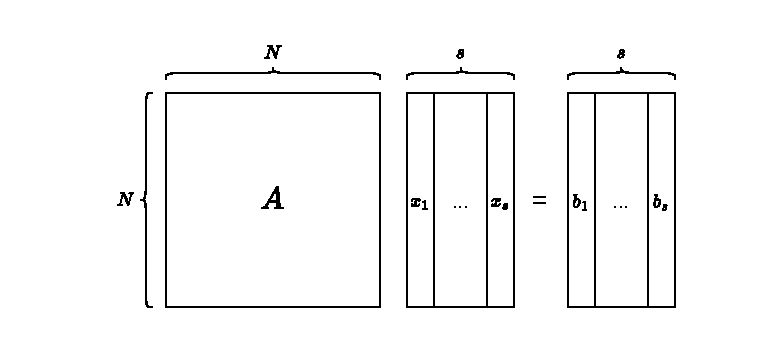
\includegraphics[width=0.5\linewidth]{images/system.pdf}
    % \caption{Caption}
    \label{fig:system}
\end{figure}
$$AX=B,$$
где $A$ - $N\times N$ невырожденная разреженная матрица системы;
$B$ - $N\times s$ невырожденная матрица, столбцы - правые части; 
$X$ - $N\times s$ матрица, столбцы - решения для соответствующих правых частей. 
Также еще предполагаем, что $s\ll N$.
Такие задачи можно решать прямыми методами, однако они не подходят для больших 
задач из-за кубической сложности. Так что естественным является использование 
блочных крыловских методов.\\

\par В преимущества блочных крыловских методов входят:
высокая производительность на вычислительных системах за счет блочных операций,
Более быстрая сходимость, по сравнению с неблочными методами \cite{OLEARY1980293}; 
в задачах со структурированными системами (например МКЭ) БКМ не разрушают структуру,
в отличие от прямых методов.
Чрезвычайно большие системы, которые не помещаются целиком в оперативную память 
можно решать с помощью блочных крыловских методов.\\
\par <Рассказ про блочные крыловские методы.>\\
\par Для наших целей мы хотим построить крыловские методы, отвечающие следующим требованиям: методы должны находить
решения систем общего вида, то есть, которые не обязательно являются эрмитовыми;
% (в отличие, например, от CG, который работает только для эрмитовых систем); 
методы не должны требовать сохранения всего крыловского пространства, то есть должны 
давать короткие итерационные соотношения; 
% (в отличие от, например, GMRES)


\newpage
 %% Введение
    % \input{parts/Chapter1.tex} %% Постановка задачи
    \section{Крыловские методы решения систем уравнений}
\label{sec:Chapter2} \index{Chapter2}

Здесь надо рассмотреть все существующие решения поставленной задачи, но не
просто пересказать, в чем там дело, а оценить степень их соответствия тем
ограничениям, которые были сформулированы в постановке задачи.

\subsection{Метод сопряженных градиентов}
[YOUSEF SAAD ITERATIVE METHODS FOR SPARSE LINEAR SYSTEMS SECOND EDITION]
\subsection{Метод бисопряженных градиентов}
[YOUSEF SAAD ITERATIVE METHODS FOR SPARSE LINEAR SYSTEMS SECOND EDITION]
\subsection{Метод стабилизированных бисопряженных градиентов}
[VAN DER VORST BI-CGSTAB: A FAST AND SMOOTHLY CONVEGRING VARIANT OF BI-CG FOR THE SOLUTION OF NONSYMMETRIC LINEAR SYSTEMS]
\subsection{Метод блочных сопряженных градиентов}
[DIANNE P. O'LEARY THE BLOCK CONJUGATE GRADIENT ALGORYTHM AND RELATED METHODS]
\subsection{Метод блочных бисопряженных градиентов}
[DIANNE P. O'LEARY THE BLOCK CONJUGATE GRADIENT ALGORYTHM AND RELATED METHODS]
\subsection{Метод блочных стабилизированных бисопряженных градиентов}
[GUENNOUNI A BLOCK VERSION OF BCGSTAB FOR LINEAR SYSTEMS WITH MULTIPLE RIGHT-HAND SIDES ]
\subsubsection{Матричнозначные полиномы}
 \par Проблемы со сходимостью метода из [GUENNOUNI], демонстрация в 4 главе, решение проблемы в 3 главе.
 \subsubsection{Алгоритм}


\newpage
 %% Обзор существующих решений
    \section{Исследование и построение решения задачи}
\label{sec:Chapter3} \index{Chapter3}

\subsection{Реортогонализация для поддержания биортогональных соотношений}
$\alpha, \beta, \omega$
\subsection{Ортогонализация векторов направлений и проверочных невязок}
$P_k = Q_PR_P$\\
\par $\tilde{R}_0$\\

\subsection{Выбор правых частей}
график с сингулярными числами
\par rrqr
\subsection{Проблемы}
Нескалярная омега
\par возможные брейкдауны [GUENNOUNI]
\par Все равно мало правых частей

\newpage
 %% Исследование и построение решения задачи
    \section{Модификация блочного симметричного метода квазиминимальных невязок}
\label{sec:bsqmr_mod} \index{bsqmr_mod}

\par Один из ключевых элементов блочного симметричного метода квазиминимальных невязок \cite{doi:10.1137/0917019}
является процесс Грамма-Шмидта с квазискалярным произведением. Далее будет представлена модификация 
этого алгоритма, использующая настоящее QR-разложение. Тогда откроется возможности для более устойчивых реализаций
QR-разложения и их библиотечным реализациям, а также к нескольким новым свойствам невязок.

\par Блочный симметричный процесс Ланцоша приводит к следующему матричному соотношению:
\begin{equation}
    \label{eq:bsqmr_AVeqT}
    A \begin{pmatrix}
        V_1 & ... & V_k & V_{k+1} 
    \end{pmatrix} = \begin{pmatrix}
        V_1 & ... & V_k & V_{k+1} 
    \end{pmatrix} \begin{pmatrix}
        \alpha_1 & \delta_1 & & & \\
        \beta_2 & \alpha_2 & \delta_2 & & \\
        & \beta_3 & \ddots & \ddots & \\
        & & \ddots & \alpha_{k-1} & \delta_{k-1} \\
        & & & \beta_k & \alpha_k \\
        & & & & \beta_{k+1}
    \end{pmatrix},
\end{equation} 
где $\delta_{i-1} = \beta_i^T$ в версии из статьи \cite{doi:10.1137/0917019}, в нашей
модификации же получится другой вид для этой матрицы коэффициентов. Из \eqref{eq:bsqmr_AVeqT} для $k$-го блока следует: 
\begin{equation}
    \label{eq:bsqmr_last_block}
    AV_k = V_{k-1}\delta_{k-1} + V_k \alpha_k + V_{k+1} \beta_{k+1}
\end{equation}

При построении базиса в блочном крыловском пространстве, требуется выпонение следующего свойства:
\begin{equation}
    \label{eq:VTVeq0}
V_i^TV_j=0,\;i \neq j
\end{equation}  

Домножая слева выражение \eqref{eq:bsqmr_last_block} на $V_{k-1}^T$ и используя соотношение
\eqref{eq:VTVeq0} получаем системы линейных уравнений на матрицу $\delta_{k-1}$:
\begin{equation}
    \label{eq:delta_system}
    V_{k-1}^T V_{k-1} \delta_{k-1} = V_{k-1}^T A V_k.
\end{equation}

Сделав замену в \eqref{eq:bsqmr_last_block} вида $k \rightarrow k-1$ и учтя выражение 
\eqref{eq:delta_system} выразим $\delta_{k-1}$ через $\beta_k$:
\begin{equation*}
    V_{k-1}^T V_{k-1} \delta_{k-1} = \beta_{k}^T V_k^T V_k.
\end{equation*}
Введем обозначение $\gamma_k = V_k^T V_k$.

Тогда окончательный вид для $\delta_{k-1}$:
\begin{equation}
    \label{eq:delta_final}
    \delta_{k-1} = \gamma_{k-1}^{-1} \beta_k^T \gamma_k.
\end{equation}

Аналогично $\delta_{k-1}$ из \eqref{eq:bsqmr_last_block} получим системы линейных
уравнений на $\alpha_k$:
\begin{equation*}
    \gamma_k \alpha_k = V_k^T A V_k.
\end{equation*}
И воспользовавшись свойством \eqref{eq:VTVeq0} преобразуем выражение для $\alpha_k$:
\begin{equation}
    \alpha_k = \gamma_k^{-1} V_k^T (A V_k - V_{k-1} \delta_{k-1}).
\end{equation}

Выбор $\beta_{k+1}$ является произвольным и определяется целями исследователя, в 
предлагаемой модификации $\beta_{k+1}$ выбрано таким, чтобы выполнялось соотношение
$V_{k+1}^* V_{k+1} = I$, где $I$ - единичная $s \times s$ матрица. Этого можно достичь с помощью QR-разложения:
\begin{equation}
    V_{k+1}, \beta_{k+1} \xleftarrow{QR} A V_k - V_{k-1} \delta_{k-1} - V_k \alpha_k. 
\end{equation} 
Этот выбор обладает рядом преимуществ: \begin{enumerate}
    \item получение QR-разложения в сравнении с квази-QR-разложением является более устойчивой операцией, 
    \item на первой итерации алгоритм ведёт себя как обобщённый метод минимальных невязок, что обеспечивает на первой итерации достижение точного минимума невязки в построенном к этому моменту пространстве Крылова, что в свою очередь предотвращает большие скачки невязки на первых итерациях, как это наблюдается в алгоритме из статьи \cite{doi:10.1137/0917019}.
\end{enumerate}  

Но предлагаемый алгоритм обладает и рядом недостатков:
\begin{enumerate}
    \item В задаче электромагнитного рассеяния на миндалевидном теле, дискретизированном методом интегральных уравнений \cite{stavtsev2009application} метод не сходится до требуемого порога в арифметике с одинарной точностью. 
\end{enumerate}

Окончательный вид алгоритма:
\begin{algorithm}
    \caption{Модифицированный блочный симметричный метод квазиминимальных невязок}\label{alg:bsqmr_mod}
    \begin{algorithmic}
        \State $V_0 = P_{0} = P_{-1} = 0_{N \times s}$, $N$ - размер матрицы $A$, $s$ - количество правых частей.
        \State $c_0 = b_{-1} = b_0 = 0_{s \times s}$
        \State $a_0 = d_{-1} = d_0 = I_{s \times s}$
        \State $R_0 = B - AX_0$
        \State $V_1,\; \beta_1 \xleftarrow{QR} R_0 $
        \State $\gamma_{0} = I_{s \times s}$
        \State $\gamma_{1} = V_1^T V_1$
        % {\color{red}
        % \State $\omega_{-1} = 0_{m \times m}$
        % \State $\omega_0 = I$
        % }
        \State $\tilde{\tau}_1 = \beta_1 $
        \For {$k = 1, ... $}
            \State $\delta_{k-1} = \gamma_{k-1}^{-1} \beta_k^T \gamma_k $
            \State $\tilde{V}_{k+1} = AV_k - V_{k-1} \delta_{k-1}$
            \State $\alpha_k = \gamma_k^{-1} V_k^T \tilde{V}_{k+1}$
            \State $\tilde{V}_{k+1} = \tilde{V}_{k+1} - V_k \alpha_k$
            \State $ V_{k+1},\; \beta_{k+1} \xleftarrow{QR} \tilde{V}_{k+1} $
            \State $\gamma_{k+1} = V_{k+1}^T V_{k+1}$
            % \State {\color{red} $\omega_{k+1} = I$}
            \State $\theta_k = b_{k-2} \delta_{k-1}$
            \State $\eta_k = a_{k-1}d_{k-2}\delta_{k-1} + b_{k-1}\alpha_k$
            \State $\tilde{\zeta}_k = c_{k-1} d_{k-2} \delta_{k-1} + d_{k-1} \alpha_k$
            \State $ Q_k ,\; 
                    \begin{pmatrix} 
                        \zeta_k \\
                        0_{s \times s}
                    \end{pmatrix} \xleftarrow{QR} \begin{pmatrix}
                                        \tilde{\zeta}_k \\
                                        \omega_{k+1} \beta_{k+1}
                                     \end{pmatrix}$
            \State $\begin{pmatrix}
                        a_k & b_k \\
                        c_k & d_k
                    \end{pmatrix} \gets Q_k^*$
            \State $V_k = (V_k - P_{k-1}\eta_k - P_{k-2} \theta_k)\zeta_k^{-1}$
            \State $\tau_k = a_k \tilde{\tau}_k$
            \State $X_k = X_{k-1} + P_{k} \tau_{k}$
            \State $\tilde{\tau}_{k+1} = c_k \tilde{\tau}_k$
        \EndFor
    \end{algorithmic}
\end{algorithm}


\newpage
   
    \section{Численные эксперименты}
\label{sec:Chapter4} \index{Chapter4}

% \subsection{Тест 1}
\par Тесты производились на интересующей нас задаче – линейной системе с многими 
правыми частями, возникающей при решении задачи электромагнитного рассеяния 
методом интегральных уравнений [STAVTSEV]. Порядок системы - 14144, всего правых частей - 722.
\begin{figure}[H]
    \centering
    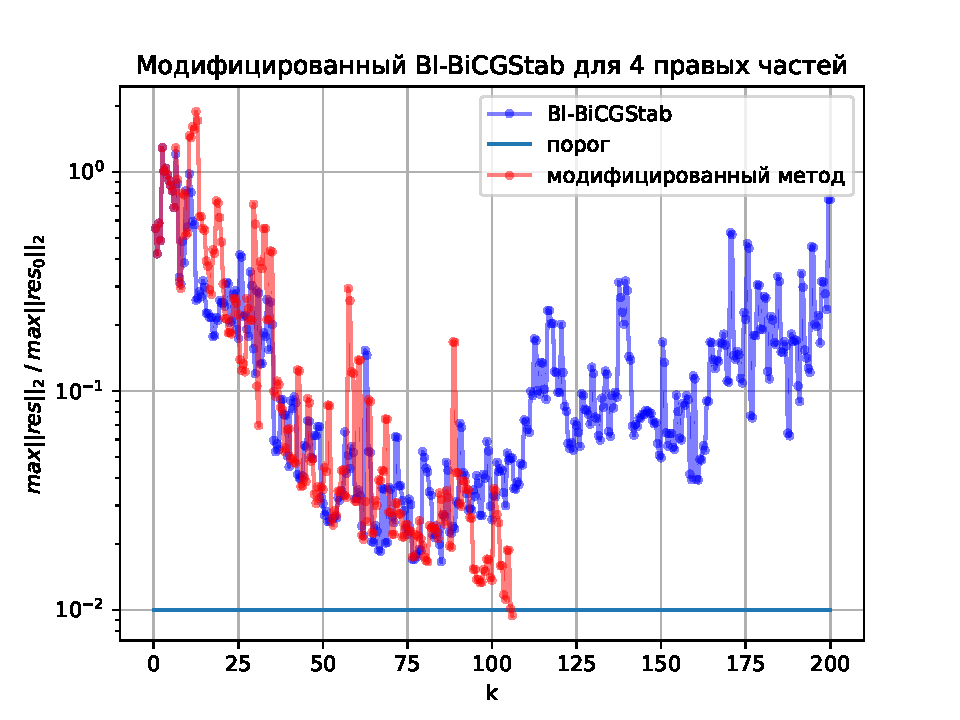
\includegraphics[width=0.7\linewidth]{images/4.pdf}
    \caption{}
    \label{fig:4}
\end{figure} 
\par Первый тест демонстрирует, что метод из статьи [GUENNOUNI] не сходится с требуемой точностью, в то время как 
версия с улучшениями, описанными в главе \ref{sec:Chapter3}, сходится линейно без проблем. 
Эксперимент проводился в одинарной точности для четырех правых частей с номерами: 0, 90, 180, 270. Его результаты представлены
на рис.\ref{fig:4}
% \subsection{Тест 2}
\begin{figure}[H]
    \centering
    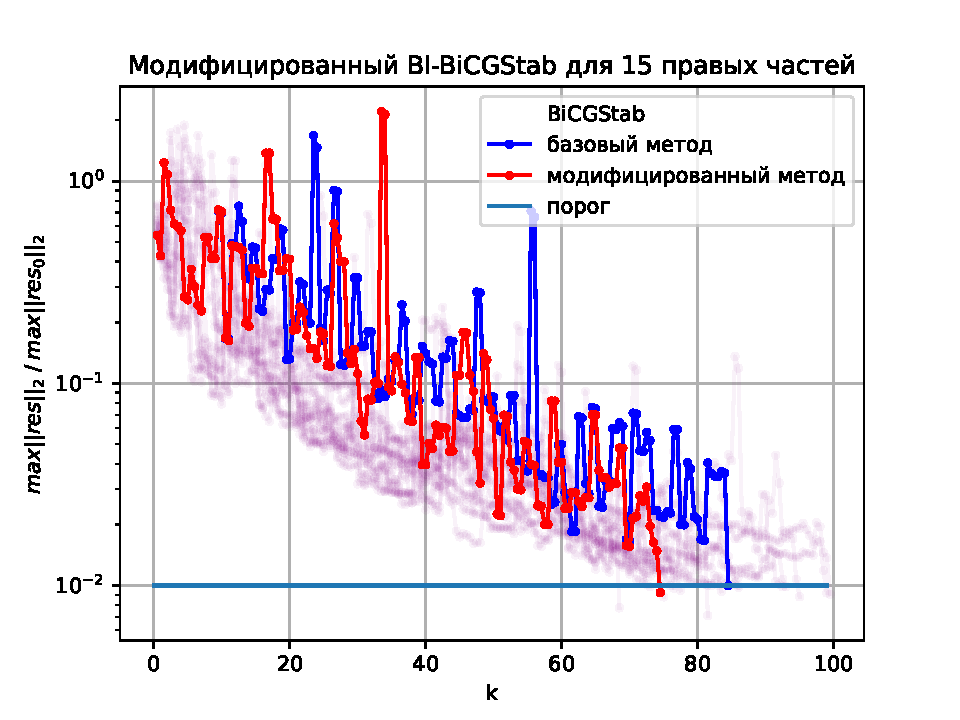
\includegraphics[width=0.7\linewidth]{images/acceleration_15_rhs.pdf}
    \caption{}
    \label{fig:acceleration_15}
\end{figure}
\par 15 правых частей, уменьшения числа итераций, считаем в двойной точности
\par Второй тест демонстрирует, что улучшения, описанные в главе \ref{sec:Chapter3} позволяют получить ускоренную сходимость
по сравнению с решением систем с каждой правой частью в отдельности
% \subsection{Тест 3}
\par более 30 правых частей, демонстрация отсутствия взрыва невязки

\newpage
 %% Описание практической части
    \section{Заключение}
\label{sec:Chapter5} \index{Chapter5}

Результаты\\
\par Нерешенные проблемы редукции блока\\


\newpage
 %% Заключение

    %% НЕ ТРОГАЙТЕ!!!
    \nocite{*}
    \bibliography{references}

    %% в зависимости от надобности подключаем раздел "Приложение"
    % \newpage
    % \input{Appendix.tex}
\end{document}
